\chapter{Project Plan}
This section is an excerpt of the project plan. The project plan features descriptions of which experiments, technologies etc. to conduct, investigate and implement during the Bachelor's Project. \newline

This section contains how the project work will be structured, which methods to be used, etc. \newline

\subsection{The Bachelor's Project}
The Bachelor’s Project (Thesis or Final Project) is an extensive project dealing with a realistic engineering assignment. The bachelor project should document the students’ ability to work independently to apply engineering methods and theories in solving professional problems and development issues in a specific field. The project constitutes the conclusion of the programme and is placed in the last semester. \newline

The Bachelor's Project workload is \textbf{20 ECTS points}. \textbf{1 ECTS} translates to \textbf{27 hours of workload}, totaling \textbf{540 hours} of workload for the Bachelor's Project. Assuming 18 weeks of Bachelor's Project work, total workload/week is ~30 hours/week. \newline

During the project period, 2 elective courses with 10 ECTS points in total to fulfill the goal of 30 ECTS workload each semester. Assuming 18 weeks of lectures and homework assignments and projects, total workload/week is ~16-17 hours/week. \newline

Total workload is therefore expected to be ~45-50 hours/week during the semester. To keep track of the project, weekly SCRUM meetings with supervisor is essential along with project management tools: \\

- The ASE-model \\
- SCRUM \\
- Redmine \newline

\subsection{ASE-model}

\begin{figure}[H]
\centering
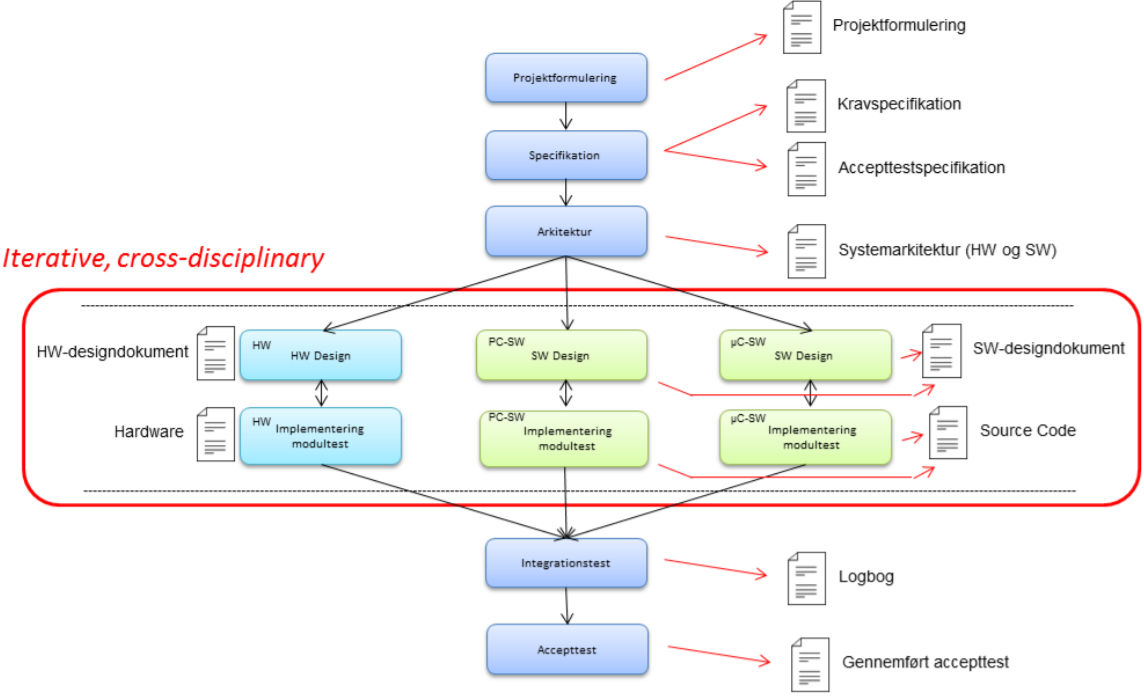
\includegraphics[scale=0.4]{./pictures/ASEmodel.png}
\caption{The Aarhus School of Engineering model - The ASE-model.}
\label{fig:ASEmodel.png}
\end{figure}

The figure above is the ASE-model that engineering students at Aarhus School of Engineering (ASE) was introduced to during their 2nd semester. The ASE-model is a structured model for design and development of hardware- and software-systems. \newline

A project of this magnitude contain and introduce several new technologies, with it many technical and project risks during the project work. Thus, an iterative project procedure is a helpful tool to ensure a clear procedure, as the beginning a new projects is usually difficult, necessitates management and overview to prevent wasting time on unnecessary activities. \newline

The iterative, cross-disciplary model is useful when designing domain, technology, implementation possibilities, etc. Designing a system using the ASE-model reduces possible project risks and enables the option to specify requirements, formulate tests and design complete use-cases early in the project. Combining the ASE-model with an iterative process, the project process is robust from project risks and future modfications. \newline

An iterative process produces functional product parts by completing tasks \textit{piece by piece} (iterations) for each module of the project. Using this method, an early assessment of project success is possible along with an early risk prevention assessment. \newline

Every iteration contains elements from several processes outlined in the ASE-model. Hence, an iteration can contain both design, implementation and test for a minor part of the project. \\

\subsubsection{Iterative development with the ASE-model}
Even though a team chooses an iterative process, the project still has various phases as shown in Figure ~\ref{fig:ASEmodel.png}. The first iterations' focus is primarily a description of idea and establishing project requirements. The following iterations focuses on system development before moving on to implementation. \\
The difference between an iterative process and the ASE-model in Figure ~\ref{fig:ASEmodel.png} is that we operate in \textit{parallel} on several types of tasks within a given iteration. This is ongoing to better build, modify and refine the product on the basis of experiences and discoveries from earlier iterations. \newline

For instance, the initial iterations outlines the first and the most important project requirements. When the reuirements are established, the problem domain is investigated: 'How can we implement GUI on a PC laptop?', 'How to measure Total Harmonic Distortion (THD) on audio output?, 'How do we establish USB-connection between GUI and Showman?', etc. \\
This iteration helps clarifying the thesis statement and allows the team the opportunities to conduct physical tests. \newline

In each iteration, the team works on almost every project area. Documentation is produced during the process and needs to be regularly updated. \\ 

\subsection{SCRUM}
SCRUM is used to manage the iterative process. The reason is the welldocumented work procedures and team roles. Organizing the project by using SCRUM gives the project a clear overview and keeps the work flow going, even though external activities such as other courses can distract the process - In short, SCRUM makes the project manageable as the teams works toward small, but clear goals. Another reason is the widely accepted use of SCRUM in companies, giving the team necessary introduction and experience in using SCRUM. \newline

The project team defines a framework with a set of \textbf{milestones} with mandatory assignments for each milestone, but gives the team the freedom to reach these milestones. \newline

Even though SCRUM is an integral part of project work at ASE, a detailed analysis and discussion of SCRUM is not within the scope of this document. The following is brief overview of selected elements of SCRUM. \newline

\subsubsection{Milestones}
The table in Figure ~\ref{fig:milestonespng} below outlines the typical milestones for a project at ASE, weeknumbers relative to semesterstart:

\begin{figure}[H]
\centering
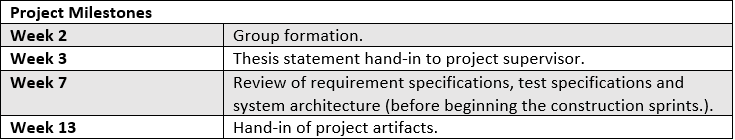
\includegraphics[scale=0.8]{./pictures/milestones.png}
\caption{Example of SCRUM milestones.}
\label{fig:milestonespng}
\end{figure}

\subsubsection{Iterations}
The ASE guide to development process for semesterproject 3 from Blackboard suggests following iterations for project completion. The first iterations primarily outlines the overview of the project. Later iterations outline hardware production and software-coding. \\

\subsubsection{Iteration 1: Project Description (1 week)}
The first project phase establishes clear overview of project idea, the most important requirements and the most significant technical risks: \newline 

\textbf{Project Description:} Project description outlines the project idea along with a rich picture. Goals corresponding requirements are set. MoSCoW-analysis is included to identify and prioritize system requirements. \\
\textbf{Requirement Specification:} Essential `Must have'-requirements is selected for informal, brief use cases and their corresponding non-functional requirements. \\
\textbf{System Architecture:} Description of domain model based on Use Cases selected from the first iteration. A general risk assessment on system level is investigated. The assessment identifies technical risks critical for project: Unidentified interfaces, unidentified programming frameworks, unknown technology, etc. \\
\textbf{Project Plan:} A rough estimate of project plan, milestones and iterations.

\subsubsection{Iteration 2: Identification and reduction of risks (2 weeks)}
This iteration identifies risks and investigates the possibilites to reduce them by outlining the problem domain and which technologies and methods to include in the project work.
Problem domain, architecture, code, hardware, algorithms, etc. are investigated to assess risks. This helps the next iteration  of the requirement specification to be more precise and detailed. \\

\textbf{System Architecture:} This phase begins with an analysis of necessary hardware and software to reduce risks. The phase ends with a sketch of the system's general architecture such as block diagrams (BDDs), general internal block diagrams (IBDs) and identification of internal interfaces with sequence diagrams and system sequence diagrams. Initital application model for each CPU in the system is outlined based on the initial Use Cases. Application model in this iteration include a class diagram for each CPU for each CPU with boundary-, control- and domain classes. \\

\textbf{Implementation and Test:} Defining design and implementation of design with mock-ups, evaluation boards, virtual machines, emulators etc. to achieve the proof-of-concept and determine the chosen architecture's usefulness. \\

\textbf{Requirement Specification:} This phase finished by updating and clarification of requiremenents. Essential use cases are updated to fully dressed use cases and non-functional requirements i.e. external interfaces is clarified. \\

\textbf{Project Plan:} Is updated based on this phase.

\subsubsection{Iteration 3: Early Implementation and Stabilizing Requirements (2 weeks)}
This phase shift focus from establishing domains to design and implement a solution that meet the requirements based on use cases and non-functional requirements. The project is still in its early stage and many elements will most likely be modified during this iteration. \newline

This edition of the system is the bare-bone version. This phase outlines a risk assessment, risk addressing and risk minimizing and stabilization of requirements. \\

\textbf{Requirement Specification:} This phase is conluded with a revision and clarification of initial and new requirements - They are apt to be relatively stable at this point. \\

\textbf{System Architecture:} This phase contains an analysis of the most necessary implementation(s). This results in an update of System Architecture with BDDs, IBDs, descriptions of internal interfaces and SW-architecture. Following this phase, the System Architecture is apt to be relatively stable. \\

\textbf{HW/SW Design Specifications:} The selected requirements are implemented in a design and undergoes a Module Test. \\

\textbf{Project Plan:} Is updated based on this phase. \\

\subsubsection{Iteration 4-(N-1): Production of Project (2 weeks)}
This phase focuses on production of the systen: Design, implementation and test to meet requirements. The requirements are selected and prioritized from theis business value. \newline

This iteration lasts 2 weeks. First step is planning of assignments that are to be solved \textit{completely} during the sprint: Task-specific system components is designed, implemented and module testes. This iteration integrates system components. \newline

A clear-cut goal for this iteration is advantageous; it is a lot more satisfying and rewarding to have minimal, but functional GUI than to implement 10 percent of the complete, comprehensive system. \\

\textbf{Requirement Specification:} Is updated if necessary. They are usually minor updates at this stage of the project. \\

\textbf{System Architecture:} Is updated if HW/SW architecture and interfaces are modified. Architecture modifications and additions to the system components and their integrations are documented. \\

\textbf{HW/SW Design Specification:} Discoveries from previous helps modifying requirement design. Design modifications and additions to the system components and their integrations are documented. \\

\textbf{Implementation and Test:} The fabricated system components is implemented and tested - Both as isolated modules and system integrated modules. \\

\textbf{Project Plan:} No modifications of project plan unnecessary. The iterations are final; the \textit{content} might be flexible, but \textit{duration} is not modified. \newline

\subsubsection{Iteration 5: Project Hand-in (1-2 weeks)}
This final iteration concludes implementation and project documentation. The product and documentation is now ready for hand in. \\

\textbf{Requirement Specification:} Is updated and completed. \\

\textbf{System Architecture:} Is updated and completed. \\

\textbf{HW/SW Design Specification:} Is updated and completed. \\

\textbf{Implementation and Test:} Implementation and test concludes. Project parts that did not meet deadline is removed from project. \\

\textbf{Project- and Process Report:} Is finalized. \\

\textbf{SCRUM roles}
This project is a one-man project, thus an outline of SCRUM roles are redundant as they are all taken care of by one person. \\

\subsection{Redmine}
The online platform Redmine is typically used for SCRUM and project management at ASE projects to keep track of project events. Team member(s) can monitor tasks, where progress, `burndown' for tasks is presented visually with Issues Burndown or Gantt diagrams. \newline

As this project is a one-man team, the SCRUM roles are more fluid thus organized work flow and supervisor meetings are essential for the project to succeed. \\

\subsection{Supervisor Meetings}
Supervisor meetings are essential to this project as it is a one-man project. The supervisor will assist in keeping track of progress: \\
- Preliminary project plan. \\
- Gives feedback on detailed project plan. \\
- Organization and conduct ongoing supervision during the project to ensure project conclusion within given time frame. \\
- Gives continuous feedback on documentation content. \newline

The supervisor is useful when conducting review- and retrospective meetings to track progress and reflections of sprints. \newline

\subsection{Timetable}
The following Figure ~\ref{fig:timetable.png} outlines the time table for the project. They are subject to be modified during the first week of the process and after initial meeting with supervisor.

\begin{figure}[H]
\centering
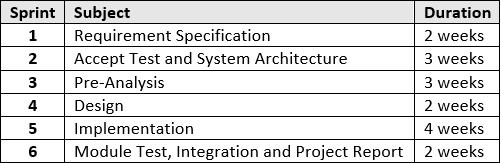
\includegraphics[scale=0.9]{./pictures/timetable.png}
\caption{A table of number of sprints and their duration.}
\label{fig:timetable.png}
\end{figure}

%\textbf{Objective} \\
%The objective of the Bachelor’s Project is that students be able to plan and conduct an engineering project in as realistic a form as the study environment allows, preferably in cooperation with companies. \\

%\textbf{Learning Objectives} \\
%Upon completion of the Bachelor’s Project, the student should be able to: \\

%- Apply scientific research results and technological knowledge for solving  technical problems, \\
%- Develop new solutions, \\
%- Acquire and evaluate new knowledge within relevant engineering fields, \\
%- Systematically apply engineering knowledge, theories and methods \\
%- Plan and complete a project in a group in cooperation with internal and external partners \\
%- Present results of a project in writing and orally by means of relevant communication tools, to professionals as well as customers, \\
%- Present results of a project orally and with means of various audio or visual communication tools, \\
%- Integrate social, economic, environmental and work environmental consequences in the solution model \newline

%Learning objectives in relation to the specific subject and with reference to above, including their weight, is specified in the Assignment Formulation. \newline

%\textbf{Main Content} \\
%The Bachelor’s Project should comprise the planning and documentation of solutions for a realistic engineering project or defined parts and comprise independent experimental, empirical and/or theoretical discussions and computations. \\

%\subsection{Project Plan}
%Project management tools are needed for the project to keep focus. Aarhus School of Engineering development model 